\documentclass[11pt]{article}
\usepackage[utf8]{inputenc}
\usepackage{amsmath}
\usepackage{amsfonts}
\usepackage{amssymb}
\usepackage{graphicx}
\usepackage[super]{nth}
\usepackage{amsthm}
\newtheorem{theorem}{Theorem}
\newtheorem{objective}{Objective}
\newtheorem{model}{Model}


\makeatletter
\renewcommand{\maketitle}{
\begin{center}

\pagestyle{empty}
\phantom{.}  %necessary to add space on top before the title
\vspace{3cm}

{\Huge \bf \@title\par}
\vspace{2.5cm}

{\LARGE Marcel Gietzmann-Sanders}\\[1cm]

{\Large\@date}

\vspace{2.5cm}
{\Large Dr. Andrew Seitz}\hspace{2cm}{\Large Dr. Curry Cunningham}\\[2cm]{\Large Michael Courtney, M.S.}\\[2cm]
College of Fisheries and Ocean Sciences\\
University of Alaska Fairbanks


\end{center}
}\makeatother


\title{Master's Research Proposal (IN PROGRESS)}

\date{2024}
\setcounter{tocdepth}{2}
\begin{document}
\maketitle
\newpage

\section{Navigating This Document}

This document is organized in order to allow you, the reader, to read as little or as much as you need/want. \newline

It begins with the \textbf{objectives} so that you know immediately exactly what this proposal is hoping to achieve and whether this is of interest to you.  \newline

Then it dives into how we will go about demonstrating success along those objectives, this will inform you on the specific \textbf{outcomes} to be expected. \newline

Finally there is a \textbf{timeline} provided to give a sense of when these outcomes can be expected. \newline

If these are compelling enough there is no need to read any further. \newline

However if you are interested in the rationales behind these objectives or diving into related work has already been done by others, the \textbf{Rationale} and \textbf{Related Work} sections are for you. 

\newpage


\tableofcontents
\newpage

\section{Objectives}

The ultimate objective of this research is to provide a new pathway by which collections of high resolution spatio-temporal movement data that are representative of a species can be used to make a direct impact on fisheries management. It is hoped that this will provide an incentive for creating/enlarging such datasets. 

\begin{objective}
To provide tooling that allows for using machine learning methods to fit models of the form

$$\psi_k = G(\eta_k)$$

that maximize the following objective:


$$\mathcal{L}=\prod_i P'(v_i | \eta_i)$$

where:

$$P'(v_i|\eta_i) = \frac{\psi_i}{\sum_k \psi_k}$$

These models will be known as odds models as they predict the "odds for" each outcome $v_k$ given the information contained in $\eta_k$. 

\end{objective}

\begin{objective}
To provide tooling that allows for running spatio-temporal simulations of management strategies using movement models as defined above. Such simulations should allow for:

\begin{enumerate}
\item Flexible initial assumptions that capture heterogeneity in the stock.
\item The ability to impose spatio-temporal mortality (both fishing and natural).
\item The ability to capture heterogeneity in fishing vulnerability.
\end{enumerate}

Likewise these simulations need to be quick enough to allow for capturing uncertainty in initial conditions through bootstrapping.\newline

These simulations will be known as diffusion models as they model the probabilistic behavior of cohorts as opposed to individual fish or schools. 
\end{objective}



\newpage


















\section{Demonstrations}

Our demonstrations of the above objectives will be split into two chapters. 

\subsection{Chapter 1}

Chapter 1 will be concerned with demonstrating the tooling for creating odds models for spatio-temporal movement behavior. It will pursue two specific modeling examples:

\begin{model}
A depth occupancy model for Chinook salmon in the Gulf of Alaska (GOA). \newline

\textbf{Target:} Depth range. \newline

\textbf{Features:} Environmental data derived either from environmental simulations or from remote sensing such as Google Earth, cohort data about the fish themselves, and temporal features such as month, season, or time of day. \newline

\textbf{Data:} PSAT tagging data from the GOA. \newline 

\textbf{Purpose:} To study the heterogeneity in depth occupancy as a function of cohort, environment, and time.  
\end{model}

\begin{model}
A movement model for Chinook salmon in the Gulf of Alaska (GOA). \newline

\textbf{Target:} Spatial grid cell selection as movement. Any state feature updates needed to capture internal states of a cohort. \newline

\textbf{Features:} Environmental data derived either from environmental simulations or from remote sensing such as Google Earth, cohort data about the fish themselves, temporal features such as month, season, or time of day, and internal state information about the cohort. \newline

\textbf{Data:} PAST tagging data from the GOA. \newline

\textbf{Purpose:} To study the heterogeneity in spatial movement/preference as a function of cohort, environment, and time.\newline

\end{model}

In building these models our primary purpose is to demonstrate the tooling exists to prudently build odds models. We can frame this goal in terms of a "standard" machine learning pipeline and work-flow. 

\begin{enumerate}
\item Formatting Data for Odds Modeling 
\item Class Balancing
\item Splitting Data into Train, Validation, Test
\item Training and Hyperparameter Tuning Using Standard Model Types
\item Diagnoses of Fit and Comparison of Different Model Types
\item Identifying Sample Groups that are More or Less Fit
\end{enumerate}

We will want to explicitly demonstrate each of these processes, provide guidance on using the tools for them, and use them to build the models listed above. \newline

The outcome will be a package in Python for building, diagnosing, and running odds models.

\subsection{Chapter 2}

Chapter 2 will be concerned with taking these models for Chinook in the Gulf of Alaska and building a spatio-temporal movement simulation that can be used to investigate a series of management questions. It is worth noting that we will use the simulation to ask questions that may come up in general management settings even if they may not be directly applicable to the issues currently faced by Chinook management in the GOA. This is just to demonstrate general applicability. \newline

The overview of the components of this simulation are outlined in Fig. \ref{fig:simulation}. Boxes with rounded edges would be inputs specified by the user. The hexagons are functions provided by the simulation and the trapezoids are data generated during the main loop. 

\begin{figure}[h!] 
  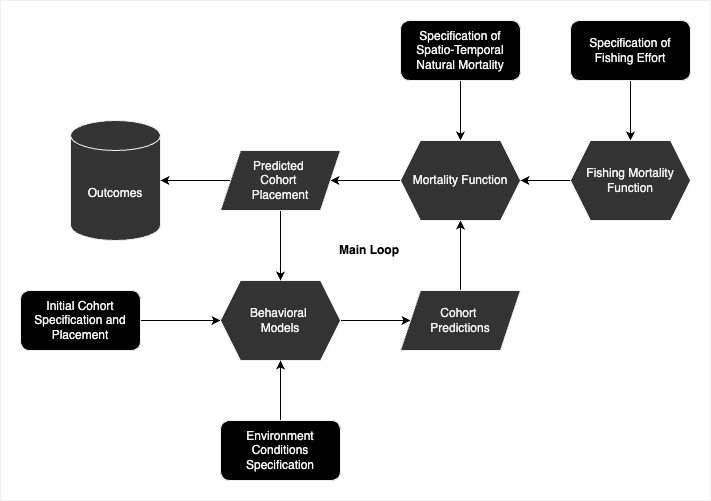
\includegraphics[width=\linewidth]{simulation.png}
  \caption{Simulation Outline}
  \label{fig:simulation}
\end{figure}


With this simulation we will attempt to demonstrate the following:

\begin{enumerate}
\item \textbf{Connectivity:} by looking at the vector flows of fish throughout the space we will be able to identify which areas are highly connected and which are more or less separated by environment, cohort, or other factors of fish behavior.
\item \textbf{Vulnerability:} by especially looking at changes in depth occupancy and preference for habitat we will attempt to quantify the degree of vulnerability in different parts of the space. 
\item \textbf{Cumulative Mortality:} we would like to demonstrate that we can model the effect of fishing the same cohorts through space as opposed to distributing the fishing mortality across more of the stock. 
\item \textbf{Protected Areas/Times:} we will attempt to demonstrate that we can simulate the effects of MPA or other kinds of closures in space and time. 
\item \textbf{Cohort Bias:} we will show (models willing) that we can understand and model differences in the above by cohort.
\item \textbf{Uncertainty:} we will show that such a simulation can be run at scale, bootstrapping can be applied, and therefore uncertainty in simulation outcomes quantified. 
\end{enumerate}

The outcome will be a package in Python for deploying, running, and analyzing diffusion models. 





\newpage



\section{Timeline}

\subsection{Class Work}

\begin{enumerate}
\item \textbf{Fall 2023:} (University of Florida) FAS 6355c Fisheries Management, FAS 6337c Population Dynamics
\item \textbf{Spring 2024:} FISH F621 Estimation of Fish Abundance, FISH F427 Ichthyology
\item \textbf{Fall 2024:} STAT F641 Bayesian Statistics, FISH F692 Seminar
\item \textbf{Spring 2025:} FISH F631 Data Analysis in Community Ecology, FISH 699 Thesis 
\item \textbf{Fall 2025:} STAT F651 Statistical Theory I, FISH 699 Thesis
\item \textbf{Spring 2026:} FISH F626  Behavioral Ecology of Fishes, STAT F605 Spatial Statistics 
\end{enumerate}

\subsection{Thesis}

\begin{enumerate}
\item \textbf{Spring 2024:} Depth and Movement Models v0, Thesis Exploration
\item \textbf{Fall 2024:} Graduate Study Plan, Self Evaluation, Thesis Proposal, Depth and Movement Models v1
\item \textbf{Spring 2025:} Thesis Proposal Defense, Simulation v1
\item \textbf{Fall 2025:} Self Evaluation, Write Chapters, Publish Package(s)
\item \textbf{Spring 2026:} Thesis Defense
\end{enumerate}

\newpage


















\section{Rationale}

\subsection{Objective 1}

\subsubsection{Value of Machine Learning in Model Building}

One of the functions of science is to build models of the world around us. Specifically to look for functions of the form:

$$v=F(\theta)$$

where $\theta$ is some vector of information, $v$ is a particular outcome given that information, and $F$ is the model in question. This we might term a \textit{deterministic model} because for any specific $\theta$ there is one single outcome $v$. 

However, life is rarely so kind to us. From quantum physics to fisheries science the world is replete with examples where the same information does not always lead to the same conclusion. Sometimes that is because we do not possess all of the relevant information but sometimes things are just truly random. As such, the model above will in some sense be lying to us in its deterministic certainty - while we will always predict $v$, $v$ is not always what we will receive. 

Instead suppose that for a specific $\theta$ there exist a set of possible outcomes $V(\theta)=\lbrace v \rbrace$. We can define a \textit{stochastic model} as:

$$P(v|\theta)=F(v, \theta)$$ 

where now the model is predicting the probability of $v$ given $\theta$ instead of just predicting $v$ itself.

Now what is especially interesting about models of this form is the fact that in some sense for any combination of $V$ and $\theta$ they always exist. Whereas to get a deterministic model we need to know precisely what kind of information ($\theta$) we need to make a deterministic prediction, we can always make a stochastic one, even in the presence of no information. The model can always give us a correct answer, it's just a question of how useful that answer is. If you base it off of better data it will become more useful.

Unfortunately, unless we ourselves have built the part of the world we're studying, $F$ is not known to us. Instead our models are really just proposals $\hat{F}$ on what $F$ could be. This presents us with an immediate problem, how do we evaluate any specific $\hat{F}$ if we don't know $F$ itself? Well suppose we've captured a whole series of pairs of $\theta_i$ and $v_i$ where $i$ allows us to index the pair in question. Given we know $\hat{F}$ we can directly ask what the likelihood of the data we have collected is, given $\hat{F}$:

$$\mathcal{L}=\prod_i \hat{F}(v_i, \theta_i)$$

or equivalently (and more easily computed)

$$\ln \mathcal{L} = \sum_i \ln \hat{F}(v_i, \theta_i)$$

$\hat{F}$'s with higher $\ln \mathcal{L}$ (log likelihood) are better fits to the given data and as we have more and more comprehensive data those data better and better represent $F$ (see Appendix 1).

Therefore finding the "true" $F$ can be summarized with two steps:

\begin{enumerate}
\item Collect large amounts of comprehensive data.
\item Find the $\hat{F}$ that maximizes the likelihood of that data.
\end{enumerate}

All of this, however, has been conditional on the form of $\theta$ having been chosen. Obviously, the information we choose to collect and build our model with has an impact on how good the model is from a purely predictive perspective. So how can we compare the predictive power of different $\theta$? Well as we find $\theta$ that are more predictive the corresponding $F$'s will have greater and greater likelihoods $\mathcal{L}$, given the data. But this presents us with a chicken and the egg style problem - to know the value of $\theta$ we must know $F$, but to know $F$ we must have fit $\hat{F}$ which requires a reasonable amount of data to have been collected. I.e. I cannot know in advance if the data I am collecting is going to be useful or not. Instead anyone doing modeling finds themselves in the cycle illustrated by Fig. \ref{fig:model_cycle}.

\begin{figure}[h!] 
  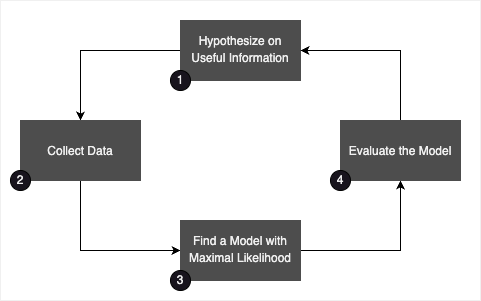
\includegraphics[width=\linewidth]{model_cycle.png}
  \caption{Modeling Cycle}
  \label{fig:model_cycle}
\end{figure}

Each step in this cycle is highly non-trivial. However special interest should be paid to step 3 (finding an $\hat{F}$ that best approximates $F$). 

The standard method here has been to propose a family of possible $F$ which are defined by a set of parameters $\mu$. Then using some choice of likelihood maximization method the set of $\mu$ are searched for that maximize the likelihood of the data $\mathcal{L}$. While this method has borne considerable fruit it still requires a great deal of effort on the side of the scientist to envision various hypotheses on what families of functions would make sense, coding those up, fitting them, and then evaluating them post-fit. Furthermore if the true form of $F$ is not contained in those set of hypotheses tested then $F$ is never found. Lots of effort without any kind of guarantee that $F$ will be discovered.  

The field of Machine Learning (ML) (specifically probabilistic machine learning) on the other hand has been specifically occupied with finding ways to maximize objectives without having to assume much, if anything, about the functional form of the prediction function. Therefore it provides an opportunity to lessen the toil and uncertainty in step 3 and allow scientists to focus more of the efforts on the other steps (and thereby accelerate the whole cycle).

\subsubsection{Issues with Probabilistic Machine Learning when Applied to Behavior}

Probabilistic machine classification of the kind we were pointing to in the last section has two pitfalls when it comes to modeling behavior. 

The first comes from the fact that such models predict on the same set of outcomes each time, regardless of $\theta$. For example, if we were trying to predict which drink a person will buy at their local cafe we would not only have to include everything currently on the menu but also everything that could be on the menu across all time points we are interested in predicting. If suddenly a new menu item appears that we have not trained on, our probabilistic classifier will be at a loss. 

The second issue comes from the "curse of dimensionality". Basically this is an issue where as the dimensionality of $\theta$ increases, the amount of data required to find real relationships in that data increases exponentially. This is a particular problem for behavioral modeling because we in all likelihood need to include data on each of the possible decisions before us. So if I can choose between 5 different drinks I need to provide features on each of those five drinks. This leads to very high dimensional spaces very quickly. \newline


We can get around both of these problems by introducing what we will term an "odds model". Specifically if we imagine $\theta$ now as a variable length vector composed of vectors $\eta_k$ for each of our possible outcomes $v_k$ then the odds model is given by the function:

$$\psi_k=G(\eta_k)$$

where we now say that:

$$P'(v_k|\theta) = \frac{\psi_k}{\sum_j \psi_j}$$

We can see why we chose the name "odds model" as the $\psi_k$ are simply the "odds for" outcome $v_k$. \newline

Now note it is not necessarily true that:

$$P'(v_k|\eta_k) = P(v_k|\theta)$$

because it is possible that information in the other $\eta_j$ informs the probability of $v_k$. However it should be possible to include such information in the $\eta_k$ if necessary. 

By making this sacrifice, however, we have achieved two things:

\begin{enumerate}
\item So long as we can provide a $\eta_k$ for a newly seen outcome we can predict on it. Therefore we need not have a fixed set of possible outcomes (or a fixed number of such outcomes per $\theta$).
\item Compared to the corresponding probabilistic machine learning classifier, if our total number of outcomes were $|V|$ we've now reduced the dimensionality of our feature space by $|V|$. 
\end{enumerate}

And this means that unless we have to pass large amounts of information between the $\eta_k$ the amount of data we need to collect to fit our model has decreased tremendously. And in cases where data is hard to come by (like animal behavior), any reduction in data requirements is of the utmost importance. 

So finally to model behavior we'd like to fit an odds model of the form:

$$\psi_k = G(\eta_k)$$

that maximizes:

$$\mathcal{L}=\prod_i P'(v_i | \eta_i)$$

where 

$$P'(v_i|\eta_i) = \frac{\psi_i}{\sum_k \psi_k}$$\newline

To the author's knowledge there is presently no tooling to fit and diagnose such models. 







\subsection{Objective 2}

From studies that started with Beverton and Holt's work on recruitment in fisheries we know, with a reasonable degree of certainty, that as a general rule fish stocks operate according to a pattern as illustrated in Fig. \ref{fig:recruitment}.

\begin{figure}[h!] 
  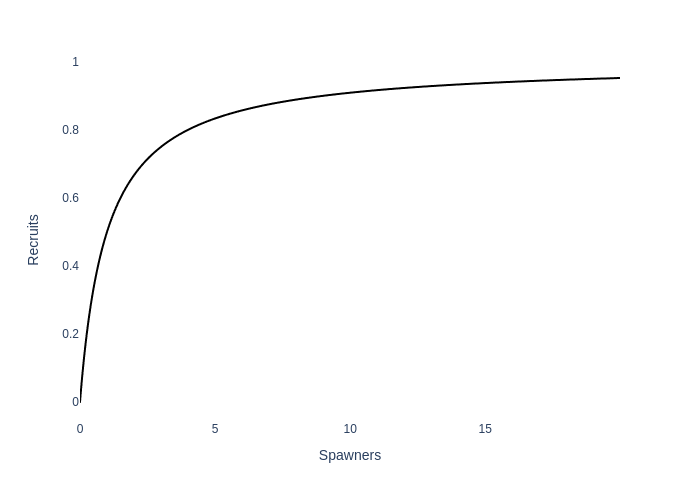
\includegraphics[width=\linewidth]{recruitment.png}
  \caption{Recruitment}
  \label{fig:recruitment}
\end{figure}

What we see is a clear pattern in recruitment verses spawners for low spawners and the eventually we reach a point where this curve asymptotes and large changes to the number of spawners creates little to no change (especially when considering the actual variability in this data) in the number of recruits. Obviously, given the real variability in nature, this pattern looks more like a scatter shot of points but plenty of studies over several species have shown this overall pattern in the mean borne out. \newline

The implication for fisheries management is pretty clear - sustainable fishing is in large part driven by just maintaining the spawning stock biomass (SSB) above that knee in the curve. Indeed this is well noted as the basis of why fisheries \textit{can} exist in the first place. If taking spawners always led to decreases in recruits, we'd quickly fish a stock out of existence. It is only through the compensation we get on the asymptote that sustainable fisheries are possible. \newline

However, two very simple observations of fish biology will show how actually managing SSB can be made difficult.

The first, and simplest, is age structure. Obviously we're talking here about maintaining a specific level of spawning stock biomass. But today's juveniles are tomorrows SSB and as fish grow they typically become more fecund. This means that in order to maintain our SSB over time we have to be careful about how we target each age group. This gets even more complicated for fish like Pacific salmon or many species of groupers where life history is intimately entwined with spawning. The salmon obviously only breed once and several species of groupers are protogynous hermaphrodites meaning that if you target a specific age group you are effectively targeting a specific sex. Clearly understanding and managing our age class selectivity matters when it comes to maintaining a healthy SSB for years to come. \newline

The other observation is that many species of fish actually form multiple sub stocks within what we may consider a single fishery (or sometimes many fisheries distributed across different countries). Pacific salmon are once again a good example in that the home to specific streams and only breed with other salmon in those streams. Bluefin tuna are also known to form specific breeding aggregations, as are many tropical fishes. Recent research too also indicates that even fish like Atlantic herring likely form distinct genetic groups due to differences in homing during breeding and school behavior. 

What does this mean? It means that if we trust our beverton-holt style model that instead of having a single SSB to manage we really have several SSB's - one for each sub stock. Obviously, if we set one global piece of management like an Allowable Biological Catch (ABC) that makes sense for a single SSB but then we have biased fishing mortality where one sub stock is getting fished out far more than the others we may drop below the SSB for that one stock without actually exceeding our expected ABC for the whole fishery. And this can certainly happen as different sub stocks will often exhibit quite different spatial behaviors in movement. \newline

All of this to say that understanding heterogeneity in vulnerability by things like age class and sub stock is of the utmost importance for managing a fisheries and truly ensuring an appropriate amount of SSB remains year over year. 

It is also worth noting that this knowledge around changes in selectivity in space and time is not only useful for considerations around SSB but also for other management issues such as bycatch avoidance and growth overfishing to name just two. 

What kind of tooling do we need in order to address these issues and test out ideas for "selectivity aware" fisheries management? Clearly we need some kind of reliable simulation. \newline

Suppose we built models of spatio-temporal behavior (specifically movement) as expressed in Objective 1. These models we know can be fed information that captures both environmental variables but also factors we'd like to categorize by in order to understand heterogeneity in selectivity. Such variables could include features like the age and genetic cohorts that we just described. Then we could take some baseline assumptions about abundance in space at a given time (say providing recruits at spawning grounds or taking a spatio-temporal assessment as a starting point) and then using our behavioral models to simulate time-steps forward. As we do these time steps we could account for natural mortality as well to complete the "environment" portion of our simulation. 

It is important to note that while this may seem like a Lagrangian approach to simulation it actually falls more into the Eulerian camp as, in order to reduce our computational costs, we'd simply have cohorts as a function of space. Remember that our model is only taking the categories that separate one group from the next thereby allowing us to model cohorts instead of single individuals. Furthermore instead of modeling the specific singular behaviors our behavior model as outlined in Objective 1 allows us to understand the "many world" probabilistic outcomes of behavior. We are not following a single fish but instead are watching as that cohort diffuses across its decision space. Therefore we'll term this simulation a diffusion model.

Into our diffusion model we can now incorporate whatever management policy we like as a spatio-temporal specification of fishing mortality - which can now be modulated by our understanding of, say, gear selectivity as a function of space and time. So if we want to implement a marine protected area we can take a baseline fishing pattern and exclude specific areas in space. If we want to see what would happen if we redistribute the fleet we can as well. If we just want to understand the selectivity biases already present we can simulate fleet patterns as they occur today. 

The point is that with such a simulation we are able to test different hypotheses of management on data driven understanding of fish behavior. 


\subsection{PSAT Data}

Pop-up Satellite Archival Tags (PSATs) are a great way of collecting behavior data. They are defined by three key properties:

\begin{enumerate}
\item \textbf{Archival:} Transmitting data is only possible if animals come to the surface. Therefore these tags archive collected data for later transmission. 
\item \textbf{Pop Up:} These tags are programmed to release from a fish at a specific time or under specific conditions to facilitate retrieval. 
\item \textbf{Satellite:} On pop-up the tags then broadcast data (usually summarized) to Argos satellites which is then relayed to a database for retrieval. Such tags usually also broadcast some positioning information which allows for direct retrieval and access to the full archived dataset.
\end{enumerate}

The normal lifecycle then is to catch an animal, attach the tag, allow the animal to go about its life all while collecting data, have the tag pop-up, transfer data to satellite or retrieve the tag, and then clean and analyze the data. \newline

For our purposes these tags critically capture:

\begin{enumerate}
\item Temperature
\item Depth
\item Light Levels
\end{enumerate}

The latter two are then used along with tag release location to predict animal movement (latitude and longitude) using a proprietary statistical model. 

We will look at movements on a day by day basis and depths at the transmitted resolution (2-5 minutes). For those tags retrieved, a much higher resolution is available (1-3 seconds) however most fish had data only from transmission and not from retrieval. 
\newline

Clearly then this kind of data suites our modeling and simulation purposes well as we get behavior outcomes directly. 

\subsection{Chinook in the GOA}

At this point in time the main interest here is that Chinook present an interesting model species for testing out the efficacy of these models and simulations. Chinook are highly motile and undergo clear migration behaviors. Therefore they should provide a good challenge to attempts at behavioral modeling and simulation. It is the author's hope that patterns useful to Chinook management issues may arise from this research but it is not a necessity as the intention here is to develop tools that justify additional data collection for species where spatial management is of interest. 





























\newpage















\section{Related Work}

\subsection{Chinook Ecology}

\subsection{Chinook Management}

\subsection{Other Applications of PSAT Data}

\subsection{Spatial Modeling}

\subsection{Spatial Assessment}

\subsection{Spatial Management}































\newpage

















































\section{Appendices}


\subsection{Value of Log Likelihood Maximization}

\begin{theorem}
Suppose we have a set of possible outcomes $V=\lbrace v_k \rbrace$ with probabilities $P_k$. Such that:

$$\sum_k P_k = P$$

Next suppose we concoct a new series of probabilities $U_k = P_k \alpha_k$ s.t. 

$$\sum_k U_k = P-\epsilon$$

where $\epsilon \geq 0$. There does not exist a set of $\alpha_k$ s.t.

$$\prod_k \left(\frac{P_k\alpha_k}{P_k}\right)^{P_kN}>1$$

\end{theorem}

\begin{proof}

We proceed by induction. \newline

First note that from the equation above we get:

$$\sum_k P_k \ln \alpha_k > 0$$

and subtracting $\sum_k U_k$ we arrive at:

$$\sum_k P_k \left( \ln \alpha_k - \alpha_k \right) > -P+\epsilon$$

Now suppose for $k$ outcomes we know no such $\alpha_k$ exist as to satisfy the above. Suppose we incorporate a new $k+1$ term s.t:

$$P_{k+1} + \sum_k {P_k} = P_{k+1} + P$$ 

and:

$$P_{k+1}\alpha_{k+1} + \sum_k {P_k}\alpha_k = P_{k+1} + P - \epsilon = P_{k+1}\alpha_{k+1} + \left(P - P_{k+1}(\alpha_{k+1}-1) \right) - \epsilon$$ 

Now we need:

$$P_{k+1}\left(\ln \alpha_{k+1} - \alpha_{k+1}\right) + \sum_k P_k \left( \ln \alpha_k - \alpha_k \right) > -P_{k+1}-P+\epsilon$$

However given our inductive assumption we know that at best, 

$$\sum_k P_k \left( \ln \alpha_k - \alpha_k \right)=-P$$

therefore at best:

$$P_{k+1}\left(\ln \alpha_{k+1} - \alpha_{k+1}\right) - P > -P - P_{k+1} + \epsilon$$

Furthermore the easiest case for us is if $\epsilon=0$. If it cannot be satisfied than this certainly doesn't work for $\epsilon>0$. So let's consider:

$$P_{k+1}\left(\ln \alpha_{k+1} - \alpha_{k+1}\right) - P > -P - P_{k+1}$$

or equivalently:

$$\ln \alpha_{k+1}> \alpha_{k+1}-1$$

Now if $\alpha_{k+1}=1$ we have:

$$\ln 1 = 1-1$$

Further consider the derivatives of each side:

$$\partial_{\alpha}\ln \alpha_{k+1}=\frac{1}{\alpha_{k+1}}$$

$$\partial_{\alpha}(\alpha_{k+1}-1) = 1$$

If $\alpha_{k+1}> 1$ then the log component rises more slowly than the constant component. I.e. our left side will be larger than the right. Likewise if $\alpha_{k+1}<1$ the log component will shrink faster that the constant component which means it will also be less than the constant component. Therefore given our assumptions:

$$\ln \alpha_{k+1} \not\ge \alpha_{k+1}-1$$

and so:

$$P_{k+1}\left(\ln \alpha_{k+1} - \alpha_{k+1}\right) - P \not\ge -P - P_{k+1} + \epsilon$$

So much for the $k+1$th case. What about $k=1$. This is trivial because any $\alpha_1$ that satisfies:

$$\sum_k U_k = P-\epsilon$$

must be less than or equal to $1$ and therefore our product of quotients:

$$\prod_k \left(\frac{P_k\alpha_k}{P_k}\right)^{P_kN}>1$$

must be less than or equal to one. 

\end{proof}


With this proof in hand we can now show how in the limit as the number of samples taken $N$ goes to infinity our likelihood is only maximized if $\hat{F} \rightarrow F$. \newline

For some given information $\theta$ and outcomes $V=\lbrace v_k \rbrace$ we have, in gathering our data, observed $v_k$ $N_k$ times. Therefore our overall likelihood is:

$$\mathcal{L} = \prod_k \hat{F}(v_k, \theta)^{N_k}$$

Now suppose that we represent:

$$\hat{F}(v_k, \theta)=F(v_k, \theta)\alpha_k$$

That is the ratio of our likelihoods between $\hat{F}$ and $F$ is given by:

$$\prod_k \left(\frac{F(v_k, \theta)\alpha_k}{F(v_k, \theta)}\right)^{N_k}$$

but we also know that:

$$\sum_k F(v_k, \theta) = \sum_k F(v_k, \theta)\alpha_k = 1$$

and that $\lim_{N\rightarrow \inf}N_k = F(v_k, \theta)N$ so that we have:

$$\prod_k \left(\frac{F(v_k, \theta)\alpha_k}{F(v_k, \theta)}\right)^{F(v_k, \theta)N}$$

which is now in the exact same form as our theorem above. And we now know that this ratio is maximized when $\alpha_k\equiv 1$. So as $N\rightarrow \inf$ a higher $\mathcal{L}$ means we are closer to approximating $F$. 


















\end{document}